
%: ----------------------- introduction file header -----------------------
\chapter{Introduction}

%\begin{flushright}
%I am just now beginning to discover the difficulty 
%\linebreak
%of expressing one's ideas on paper. As long as it 
%\linebreak
%consists solely of description it is pretty easy, but  
%\linebreak
%where reasoning comes into play, to make a proper
%\linebreak
%connection, a clearness \& a moderate fluency, is to me,   
%\linebreak
%as i have said, a difficulty of which i had no idea.
%\linebreak
%C. Darwin
%\end{flushright}
\ifpdf
    \graphicspath{{1_introduction/figures/PNG/}{1_introduction/figures/PDF/}{1_introduction/figures/}}
\else
    \graphicspath{{1_introduction/figures/EPS/}{1_introduction/figures/}}
\fi

This PhD thesis aims at proposing, developing and validating new Evolutionary Algorithm (EA) variants for solving design-optimization problems at reasonable computing cost. This is extremely useful when handling large-scale industrial optimization problems, such as in the fields of thermal and hydraulic turbomachines. The developed EA variants, enhanced with the proposed add-on features, must be able to produce high quality designs, at acceptable (according to the industrial standards) turn-around time. The later is, in fact, necessary for EAs to become a design-optimization tool routinely used in an industrial environment. To reduce the optimization turn-around time, a method which overcomes the standard shape parameterization techniques which, in real-world applications, introduce a great number of design variables, is firstly proposed. To this end, this thesis proposes and evaluates a way to use the information residing into a small number of archived designs, made available from similar successful projects worked out in the past. This leads to optimization problems with much less unknowns which can be solved using EAs at noticeably lower computing cost. The proposed method combines ``ideas'' from the theory of Knowledge-Based Systems (KBS) with the  EAs, giving rise to a fast design method, to be referred to as Knowledge-Based Design (KBD). Furthermore, the degradation in EAs efficiency/speed when used to solve ill-posed problems motivated the development of a method able to recover a great part of the efficiency loss. In this thesis, Ill-posed optimization problems are defined as the ones dealing with non-separable (section \ref{Nonsep}), and therefore anisotropic (section \ref{IllCon}), objective functions. A non-separable objective function, as opposed to a separable one, cannot be solved as N (N being the number of unknowns) separate optimization problems since the optimal value of each unknown depends on the choice of the rest. This leads to superlinear increase, with respect of N, in computational cost something that, in comparison with the linear increase for separable problems, gets more significant as N increases. Keep in mind that the majority of industrial-scale problems are, in fact, non-separable and require a great number of unknowns.  The proposed method makes use of the Principal Component Analysis (PCA) to identify directions in the design space which, if used to reformulate the design problem by introducing new design variables, would result in  non-ill-posed optimization problems.  This information is, then, used to modify the evolution operators, leading to more efficient search.  A by-product of the aforementioned method is the assignment of ``importance'' to each design variable (or design space coordinate). Metamodel-Assisted EAs (MAEAs), in which the costly problem-specific evaluation tool (herein a CFD code) is replaced by surrogate evaluation models or metamodels (trained artificial neural networks, ANNs, polynomial regression methods, etc.), may benefit from the importance-based ranking of the design space coordinates, in order to overcome problems caused by the so-called curse of dimensionality. A method based on the truncation of the ANN entries is proposed, which leads to dependable metamodels for use during the inexact pre-evaluation phase of the MAEA performs much better.  

The aforementioned methods are validated in cases ranging from  some low-cost mathematical optimization benchmarks to 2D compressor cascade designs. Problems such as to the design of industrial 3D hydraulic turbines and the redesign of a 3D peripheral compressor cascade with tip clearance installed at LTT/NTUA have also been examined. The mathematical benchmarks have low computing cost and allow, thus, the exhaustive investigation of methods by repeating the runs, using different seeds for the random number generator, on the same case. The presented 2D cases allow the demonstration of the methods in simple aerodynamic optimization cases. Furthermore, two types of hydraulic turbines, a Francis and a new type named Hydromatrix$\circledR$, are used to validate the performance of the aforementioned methods in large-scale industrial applications. A number of performance metrics are introduced and, depending on the case, these are combined to form the necessary objectives and constraints. In the hydraulic turbomachinery design problems, more than one operating points are considered, leading to an increased cost per evaluation. Thus makes the reduction in the number of evaluations required to reach the optimal solution(s) absolutely necessary.  Finally, the blade airfoil of the 3D compressor cascade installed at LTT/NTUA, aiming at minimum total pressure losses, is optimized.     


This PhD thesis is based on EAs developed during a couple of previous PhDs \cite{phd_Giotis,phd_Karakasis,phd_Kampolis,phd_Vera} performed at the Parallel CFD \& Optimization unit of LTT/NTUA (PCOpt/NTUA). These PhD theses created the algorithmic basis or platform,  which the newly proposed methods were built upon. This EA-based platform, known as the EASY (Evolutionary Algorithm SYstem \cite{EASYsite}) includes, the basic EA, optionally enhanced by parallel search (Parallel EA or PEA), incorporation of ANNs as metamodels (MAEAs) and hierarchical optimization schemes (Hierarchical EA or HEA) provided fertile ground for the development of the new methods proposed by this PhD thesis.                       
 
%An overview of the use of optimization methods for fluid dynamic problems, a review on the previews works by PCOpt this thesis has build upon and the thesis structure follow.

\section{CFD-based Optimization}

An overview of CFD-based optimization methods is presented in this section. CFD-based optimization methods enjoy great interest (figure \ref{pubs.CFD}) from both academia and industry since the performance and, therefore, the price, of products (ranging from cars and aircrafts to thermal and hydraulic turbomachines etc.) depends heavily on their aero/hydrodynamic performance. 

\begin{figure}[h!]
\begin{minipage}[b]{1\linewidth}
 \centering
 \resizebox*{!}{8 cm}{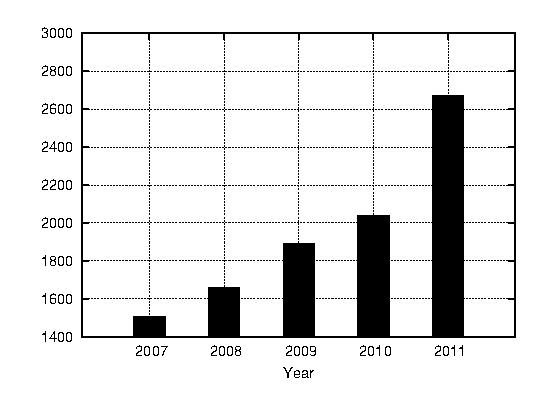
\includegraphics{OptimizationCFD.eps}}
\end{minipage}
\caption{Number of publications on CFD-based optimization appearing in ScienceDirect.} 
\label{pubs.CFD}
\end{figure}

In order to demonstrate the increasing interest of the scientific community in CFD-based optimization, an internet-based literature search was carried out using the search tool ``ScienceDirect'' (http://www.sciencedirect.com/). The search criterion was (Optimization $AND$ CFD) $OR$ (Optimization $AND$ Computational Fluid Dynamics).  This is obviously a non-exhaustive search; nevertheless it is capable to identify trends.  The steadily growing number of publications in the last five years, as seen in figure \ref{pubs.CFD}, reveals the growing interest in performing CFD-based optimization. Therefore, it is expected that the upgrades proposed by this thesis must be of interest to an increasing in size community of scientists, not necessary restricted within the field of turbomachines.     
 
A prerequisite for any shape optimization problem in fluid dynamics is the availability of a fast and reliable way to evaluate each candidate solution. This is achieved through the use of Computational Fluid Dynamic (CFD) (hence the term CFD-based optimization) methods that numerically solve the differential equations governing the fluid motion. Nowadays, thanks to the relatively cheap access to powerful computational means, the CFD tools have affordable CPU cost (depending on the case complexity) and, therefore, optimization based on them are flourishing. The strong dependence of the CFD-based optimization from the computational resources is pronounced in cases where a number of disciplines (ranging from structural analysis to manufacturing and economics) are used to evaluate the candidate solutions (multidisciplinary optimization). The fact that the fluid dynamic, structural and economical objectives may be contradictory adds extra difficulty to the optimization procedure.           
 
An important part of the optimization procedure is the definition of the design variables. An optimization algorithm seeks the value set of the design variables minimizing the user-defined cost function(s).  In CFD-based optimization typical objectives are: the maximization of lift, the minimization of drag, the maximization of efficiency, the minimization of the deviation from given target (pressure, velocity, etc.) distributions, the minimization of viscous or shock-induced losses or the cavitation index (in hydraulic turbomachines), etc.  design-optimization problems with more than one objectives (multi-objective optimization, MOO) can be solved by concatenating the objectives into a single one, after multiplying them with appropriate weights. The difficulty of choosing the most appropriate weight values and the failure of the approach in non-convex optimization problems are two of the main weaknesses of this approach.  An improved way to solve MOO problems is the use of dominance-based methods that rank the candidate solutions according to Pareto dominance \footnote{Solution $a$ dominates solution $b$ if and only if its equal to $b$, in regard to all but one objectives, and better than $b$ at list one of them.}. This method returns a set of optimal solutions forming the so-called front of non-dominated solutions or Pareto front, where none of them is dominated by any other with respect to all objectives.  Therefore, the choice of the optimal solution to be adopted relies upon additional criteria set by the decision-maker.  The design-optimization problem can, also, be subject to a number of constraints. In fluid mechanics related shape optimization, typical constraints are related to geometrical quantities (usually, thickness constraints so as to get manufacturable designs), structural quantities such as the maximum stress or deflection and/or flow-related quantities such as the minimum flow turning or the cavitation index.          

In general, CFD-based shape optimization methods can be classified in two categories, namely the direct and inverse optimization methods. Direct methods \cite{phd_Giotis,phd_Kampolis,phd:papadim,kn:Emm2002,kn:Emm2004} solve the optimization problem through a number of trials that involve the geometry generation, CFD predictions, the objective function estimation and, if necessary, its gradient computation.  On the contrary, inverse methods (should not be confused with inverse design problem \footnote{Inverse design problems use as cost function the deviation of the current from a desirable flow variable distribution.} that can be solved by direct methods) \cite{chav:95,ded:95} begin from a set of desirable flow field characteristics (such as those related to the boundary layer) and solve the inverse problem to define the geometry. The major advantage of inverse methods is their speed and their ability not to start by an initial geometry. The most noticeable drawback, on the other hand, is the inability to handle constrained optimization problems. The inverse methods developed by PCOpt/NTUA are based on the Le Foll method \cite{lefoll} which is an integral method using a two-parametric boundary layer velocity profile. This method was extended to accommodate compressibility \cite{pap69}, surface curvature effects on the turbulent boundary layer \cite{pap70} and boundary layer separation \cite{pap81} and was used for the design of both axial and radial turbomachines. Based on the above classification, this PhD thesis is dealing with direct design-optimization methods.  

Based on the characteristics of the design-optimization methods themselves,  these are classified as deterministic and stochastic ones. Deterministic methods were used first in CFD-based optimization mainly due to their solid mathematical background and fast convergence, to locate optimal solutions with less trials. The deterministic methods require the computation of the gradient of the objective function with respect to the design variables. This limits the type of objective functions such a method might handle to those being differentiable. Furthermore, the cost of the gradient calculation can be noticeably high if access to the evaluation software source code is not granted and computationally expensive finite-difference schemes must be employed. Furthermore, they have difficulties to solve MOO problems and compute fronts of non-dominated solutions with a single run and they risk of being trapped into local minima.        

In the deterministic optimization methods used in fluid dynamics design problems the most important part is the gradient calculation. The use of finite differences, as mentioned above, is not suitable since it requires, at least, as many flow analyses as the design variables. The use of adjoint techniques, though, can reduce the cost to that of a single-equivalent flow solution irrespective of the number of design variables. Due to the need of significant investment in person-months (mathematical development and programming) required for the development of the adjoint methods and software, there were not used in CFD-based optimization since the mid $80^s$ \cite{piron:84, kn:Jame88, kn:Jame94, kn:Jame95}.  The two variants of adjoint techniques, discrete and continuous, differ in the way the discretized adjoint equations are formed. The continuous adjoint method \cite{kn:Jame94, kn:Ander99,phd:papadim}, processes the flow PDEs to derive the adjoint ones which are, then, discretized. On the other hand, in the discrete adjoint variant the adjoint equations result directly from the discretized flow equations \cite{kn:Elliott96, anderson:99}. A more detailed presentation of adjoint methods used for fluid dynamic optimization can be found in \cite{phd:papadim}.        

On the other hand, stochastic optimization methods  do not suffer from the risk of getting trapped into local minima due to the probabilistic search. Furthermore, the differentiability of the objective function is not required. An additional positive feature of stochastic optimization methods, especially regarding industrial use, is their ability to handle any problem, by merely accommodating the available evaluation software, without even having access to its source code. On the other hand, their main drawback is the need to evaluate a great number of candidate solutions before reaching the optimum. This may increase, significantly the overall computational cost of the optimization procedure. This PhD thesis is dealing with stochastic optimization methods and, more precisely, with EAs. 

The use of EAs in CFD-based optimization was delayed until mid $90^s$, mainly due to their high computational cost. The first relevant works \cite{kn:Quag95,per:95,kn:Gala96} presented automated EA-based procedures for aerodynamic design-optimization problems. Soon after, emphasis was laid on the reduction of the cost of the overall optimization procedure, mainly by adapting the available variable representations and evolution operators. This continued with their hybridization with deterministic methods. For instance, in \cite{kn:Mar97} and \cite{kn:Fost97}, an EA is used to spot a good starting solution for a deterministic optimization method. In \cite{dennis:99}, EAs were hybridized with Sequential Quadratic Programming (SQP) for constrained shape optimization problems. Furthermore,  the use of distributed EAs \cite{kn:Door1997,kn:SefrThes}, surrogate evaluation models \cite{kn:Ratl98,kn:Gio99,kn:Gian1999,kn:EBNK,phd_Kampolis}, hierarchical schemes \cite{kn:Eby1998,kn:Sef2000,knowles00mpaes_x41,desideri03,phd_Kampolis} and concurrent evaluations in a multiprocessor environment  \cite{kn:LeeH96,phd_Giotis,phd_Vera} were proposed. Nowadays, the appeal of CFD optimization using EAs for industrial-scale engineering problems is increasing due to the availability of powerful computational resources. This PhD thesis is dealing with the use of EAs for solving industrial scale design-optimization problems in the fields of thermal and hydraulic turbomachines in acceptable (for the industry) turn-around time.   


\begin{figure}[h!]
\begin{minipage}[b]{1\linewidth}
 \centering
 \resizebox*{!}{8 cm}{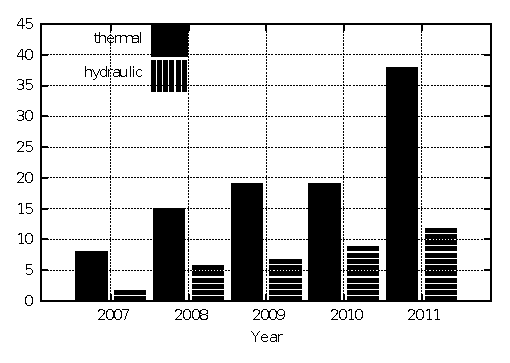
\includegraphics{hydrtherm_m.eps}}
\end{minipage}
\caption{Number of recent publications on the optimization of thermal and hydraulic turbomachines in ScienceDirect.} 
\label{pubs.turbo}
\end{figure}
 

Regarding CFD-based optimization in the fields of thermal and hydraulic turbomachines, an other internet-based literature search has been carried out as before. The search criterion where: (a) optimization $AND$ thermal $AND$ turbomachines and (b) optimization $AND$ hydraulic $AND$ turbomachines. This search reveals the steadily growing number of publications, in both thermal and hydraulic turbomachiens, over the last five years, as shown in figure \ref{pubs.turbo}. 

For instance, in the ASME 2011 Turbo Expo Conference, $24$ papers were published regarding EA-based optimization in the field of thermal turbomachines, either CFD-based or not. Most of them are handling a small number of design variables, $(N)$ up to $15$, and only three \cite{Georg2011,Marcel2011,Kevin2011} solve high dimensional problems $(N\!>\!30)$. In \cite{Georg2011}, the application of an axisymmetric endwall contour for compressors is investigated and an EA-based optimization of the outer casing and the corresponding blade tip airfoil section of a typical gas turbine high pressure compressor stage with a high number of design variables ($N\!=\!38$) is presented. In \cite{Marcel2011}, the high-dimensional ($N\!=\!210$) constrained multi-objective optimization of a fan stage, using EAs enhanced by metamodels, is presented. In \cite{Kevin2011}, an EA-based axisymmetric multi-disciplinary optimization approach for compressors is presented and applied to the design of a three-stage booster with $N\!=\!53$ design variables. Even though, the aforementioned papers use a large number of design variables, they typically start from an almost optimal design and, therefore, are able significantly restrict the design space per design variable. For instance,  \cite{Marcel2011} starts from a ``pre-optimized'' design and \cite{Georg2011} has variable's range in the tip clearance magnitude (very small). Note that the KBD method proposed by this thesis may efficiently deal with both high-dimentional ($N\!>\!300$), with extended search space per variable.      

In the IAHR 2010 conference, $5$ paper regarding optimization in the field of hydraulic turbomachines were published. Among them, three \cite{Raimunda2010,Kyriacou2010,Popa2010} used EAs. In \cite{Popa2010}, the weekly operation of a multipurpose
hydroelectric development, including a pumped storage plant was optimized using an EA. In \cite{Raimunda2010}, an optimization problem with two design variables, concerning the design of an axial compressor cascade using a MAEA was presented.  In \cite{Kyriacou2010}, the author of this thesis presented  a optimization problem with $336$ design variables concerning the design of a Francis hydraulic turbine was presented, the later was a result of this PhD thesis. 


Regarding CFD-based optimization in the fields of thermal and hydraulic turbomachines has been made in the Laboratory of Thermal Turbomachines (LTT/NTUA) and the Laboratory of Hydraulic Machines (LHM/NTUA) of NTUA. 
Concerning thermal turbomachines, a number of papers regarding both deterministic and stochastic optimization methods reflect the performed research. Most of them are related to the optimal design of components of thermal turbomachines, such as compressor cascades, using a variety of optimization methods.  An indicative subset of them is mentioned below. The use of stochastic optimization methods coupled with computational intelligence is presented in \cite{LTT_2_018,LTT_2_020,LTT_2_023}. There, the use of artificial neural networks as metamodels, in order to assist  EAs incorporating costly evaluation tools such as CFD codes, are proposed. In \cite{LTT_2_026}, the use of metamodels trained both on responses and gradients is proposed and used in the inverse design of a 3D peripheral cascade. In \cite{LTT_2_031}, the hierarchical distributed MAEA is used for the viscous loss minimization of a compressor cascade. In \cite{LTT_2_040}, an asynchronous EA is used for the optimal design of a 2D compressor cascade and in \cite{LTT_2_045} a grid-enabled asynchronous MAEA is demonstrated on the optimization of a 3D annular compressor cascade. Furthermore, in \cite{LTT_2_032}, an adjoint-based optimization method is proposed for the total pressure losses minimization in turbomachinery cascades.  In \cite{LTT_2_049},  the computation of the exact Hessian matrix of the objective function measuring total pressure losses in turbomachinery cascadesis presented for use in optimization based on Newton equation. Multilevel strategies that combine adjoint-based methods with MAEAs for turbomachines are descried in \cite{LTT_3_092}.


Concerning the CFD-based optimization in the field of hydraulic turbomachines, the work done at LHM/NTUA is related to: a) the design of optimal components of hydraulic machines, such as runner blades, and b) the optimal design of complete hydroelectric power plants and energy storage plants in combination with other forms of renewable energy generation sources, such as wind energy. Indicatively, in \cite{Anagno2}, an EA is used to improve the design of a microchannel structure, part of a valveless micropump, the so-called ``Tesla-type valve''. In \cite{Anagno4}, the fast Lagrangian approach is incorporated into an EA to design an optimal Turgo turbine. The optimal sizing of a run-of-river small hydroelectric power plant utilizing an EA is descried in \cite{Anagno3}. Furthermore, in \cite{Anagno5,Anagno6}, the optimization of pumped-storage systems for wind power plants is presented.

   

\section{EAs \& MAEAs: Previous work by PCOpt/NTUA} % section headings are printed smaller than chapter names
\label{PRW}
An overview of four previous PhD theses on EAs carried out at the same research group of the PCOpt/NTUA follows. 

Giotis's thesis \cite{phd_Giotis}, developed a generalized EA able to combine components of the two most widely used evolutionary optimization methods, namely Genetic Algorithms (GAs) and Evolutionary Strategies (ESs). Furthermore, in the same thesis or the corresponding papers \cite{kn:Emm2002,LTT_2_018,LTT_2_023}, the use of artificial neural networks as local metamodels, trained on previously evaluated candidate solutions, was proposed in order to reduce the computational burden. To reduce the wall clock time of the optimization, parallel evaluation of candidate solutions on a number of available processors, via the PVM protocol was used. The EASY optimization platform this thesis relies upon initiated from Giotis's thesis \cite{phd_Giotis}.   

Karakasis's  thesis \cite{phd_Karakasis}, further improved the EA efficiency by focusing on the optimal use of metamodels in multi-objective optimization problems. One of the most important outcomes of this thesis was that the MAEA became equally efficient in both multi- and single-objective problems, by overcoming problems related to: (a) the fact that the previously computed individuals, by the EA, in a multi-objective optimization problem, are spread along a front in the design space rather than clustered around the sought optimal solution and (b) the presence of outliers that require special treatment. Distributed EAs (DEAs) were programmed and validated, in order to increase the parallel efficiency of EAs, improve convergence and avoid stagnation during the early generations. Furthermore, the notion of Hierarchical EAs (HEAs) was introduced and this  was later refined in \cite{phd_Kampolis}.    In \cite{phd_Karakasis}, the use of a DEA on each level of the HEA associated with a different evaluation model, was proposed.

In Kampolis's thesis \cite{phd_Kampolis}, the HEAs were upgraded by introducing apart from hierarchical schemes based on the combined use of low- and high-fidelity evaluation software, other hierarchical variants making use of different parameterization schemes (coarse and fine) or different search methods allowing, thus, the combination of EAs with deterministic optimization methods. Furthermore, the introduction of artificial neural networks trained on both objective functions values and their gradient was proposed during the same thesis or \cite{LTT_2_026}.          

Part of a fourth PhD thesis, Asouti in \cite{phd_Vera}, aimed at increasing the parallel efficiency of EAs or MAEAs. This was achieved by introducing the so-called Asynchronous EA (AEAs) or Asynchronous MAEAs (AMAEAs). By utilizing a number of strongly interconnected demes, the asynchronous variants may circumvent the "end of generation" synchronization barrier and, thus, non interruptibly use all the available processors.     The proposed EA appropriate for heterogeneous multi-processor platforms. 

\section{Thesis outline} % section headings are printed smaller than chapter names
A short overview of the chapters of this PhD thesis follows:

Chapter $2$ presents the pre-existing, algorithmic basis of this PhD. This includes the generalized EA with its evolution operators, the MAEA and the HAEA.

Chapter $3$ is concerned with the first innovative method proposed in this PhD thesis, namely that referred to as the Knowledge-Based Design (KBD) one. In this chapter, a short overview of knowledge-based systems is presented. Then, the proposed KBD method is described in detail and used to perform the design of a 2D compressor cascade, in order to demonstrate its merits.

Chapter $4$ is dealing EAs and MAEAs suitable to solve ill-posed optimization problems. This chapter starts by describing the feature of ill-posed optimization problems. Then, the degradation of EA efficiency when used to solve ill-posed problems is investigated. An innovative way to find new directions in the design space that, if used to redefine the design variables, would result in a well-posed problems that can be solved using EAs and MAEAs at much less computational cost.  New evolution operators, the so-called PCA-driven ones, are devised, in order to recover the aforementioned EA efficiency loss. Furthermore, the use of the importance information, resulting form the PCA is used to enhance metamodel efficiency. Finally, the gain of the proposed methods is quantified through a 2D compressor cascade design-optimization case.

In chapter $5$, the methods proposed in this thesis are used to solve large-scale industrial problems, in the field of hydraulic turbomachines. The parameterization, grid generation and CFD tools used in this studies are presented. Quality metrics measuring each hydraulic turbine quality regarding cavitation, blade loading and draft-tube coupling are introduced. Then, the optimization of a Francis turbine, in the context of a modernization/rehabilitation project, is used to demonstrate the merits of the KBD method, by comparing it with a conventional EA. Also, the optimization of a new type of hydraulic turbine, Hydromatrix$\circledR$, is carried out in order to demonstrate the gain expected from the use of MAEAs enhanced by the proposed PCA-driven evolution operators.

Chapter $6$ is dedicated to the design-optimization of the compressor cascade installed at LTT/NTUA. This case is used to investigate the combined effects of the use of PCA-driven evolution operators and the PCA-assisted metamodels,  proposed in Chapter $4$.

Finally, Chapter $7$ summarizes the conclusions of this PhD thesis.      

%: ----------------------- HELP: references
% References can be links to figures, tables, sections, or references.
% For figures, tables, and text you define the target of the link with \label{XYZ}. Then you call cross-link with the command \ref{XYZ}, as above
% Citations are bound in a very similar way with \cite{XYZ}. You store your references in a BibTex file with a programme like BibDesk.


%%%%%%%% template for figures
%see fig \ref{A common glucose polymers}
%\figuremacro{EAvsPCA_zdt3}{A common glucose polymers}{The figure shows starch granules in potato cells, %taken from \href{http://molecularexpressions.com/micro/gallery/burgersnfries/burgersnfries4.html}{Molecular %Expressions}.}

%%: ----------------------- HELP: adding figures with macros
%% This template provides a very convenient way to add figures with minimal code.
%% \figuremacro{1}{2}{3}{4} calls up a series of commands formating your image.
%% 1 = name of the file without extension; PNG, JPEG is ok; GIF doesn't work
%% 2 = title of the figure AND the name of the label for cross-linking
%% 3 = caption text for the figure

%%: ----------------------- HELP: www links
%% You can also see above how, www links are placed
%% \href{http://www.something.net}{link text}

%\figuremacroW{EAvsPCA_zdt3}{Title}{Caption}{0.8}
%% variation of the above macro with a width setting
%% \figuremacroW{1}{2}{3}{4}
%% 1-3 as above
%% There you go. You already know the most important things.



